\section{Properties of the calculated field}
The accuracy of a simulation using a PM code depends on several factors.
The user can decide to use any combination of the following elements that parameterize the program:
\begin{itemize}
    \item mass assignment and interpolation scheme: NGP, CIC, TSC, or possibly any other scheme from the infinite hierarchy described in \autoref{sec:mass-assignment};
    \item convolution with the Green's function derived from the discretized Laplacian (\autoref{eq:dft-transformed-phi}) or the ``poor man's solver'' (\autoref{eq:poor-mans-poisson-solver});
    \item gradient approximation: two-point or four-point finite difference;
    \item grid resolution: number of meshpoints in each dimension.
\end{itemize}
In this subsection, we analyze these choices from two different angles.
We first focus on the properties of the field produced by a single source, which provides insight into the behavior of the simulation based on pair-wise interparticle interactions.
Then, we analyze the global error in force calculation by comparing the PM-calculated forces acting on all particles in a typical simulation with forces produced by the PP method.

\subsection{Local picture}
The field produced by the PM method is neither homogenous nor isotropic.
Anisotropy can be observed by measuring the field generated by a particle in two different directions.
In \autoref{fig:pm-field-properties}, the field strength calculated using the PM method (with the Green's function derived from discrete Laplacian) due to a single source at $x = H$ is shown in two variants: when measured along the $x$-axis (blue line) and the $x=y$ line (orange line).
The difference between these two graphs illustrates the anisotropy of the calculated field.
The figure also shows the field strength measured along the $x$-axis when the source was shifted by $H/2$ in the $-x$ direction (green line).
Its deviation from the case when the source was placed at $x=H$ (the blue graph) exemplifies the inhomogeneity of the field computed using the PM method.
\begin{figure}[!ht]
    \centering
    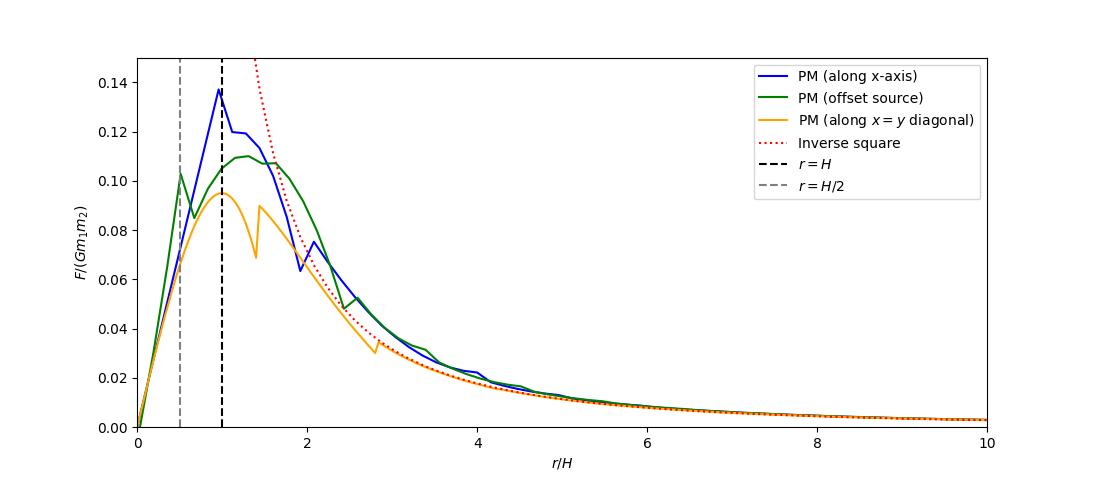
\includegraphics[scale=0.55]{chapters/pm-method/img/pm-field-combined.png}
    \caption{Anisotropy and inhomogeneity of the field as calculated by the PM method (TSC assignment, second order finite difference).}
    \label{fig:pm-field-properties}
\end{figure}
As expected, the PM-calculated approximation gets better with increasing distance from the source;
the inverse-square law is reproduced accurately for $r \gtrsim 4H$.

The single-source case analysis can be extended by considering the effect of choice of finite difference and mass assignment schemes on the relative error between the actual and approximated field strength.
\autoref{fig:pm-combined} shows a comparison of (a) the relative error as a function of distance from the source for PM with second-order and fourth-order finite differences and (b) the field strength computed using different mass assignment schemes discussed in \autoref{sec:mass-assignment}.
\begin{figure}[!ht]
    \centering
    \begin{subfigure}[t]{0.48\textwidth}
        \centering
        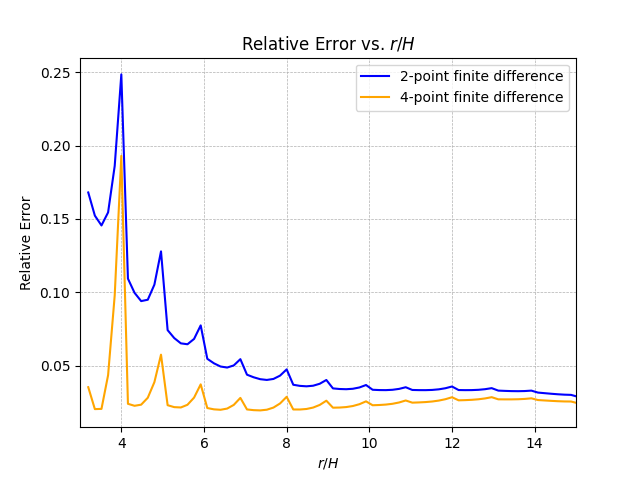
\includegraphics[width=\linewidth]{chapters/pm-method/img/pm-finite-diff-err.png}
        \caption{Relative error of field strength approximation in different finite difference schemes.}
        \label{fig:pm-finite-diff-err}
    \end{subfigure}
    \hfill
    \begin{subfigure}[t]{0.48\textwidth}
        \centering
        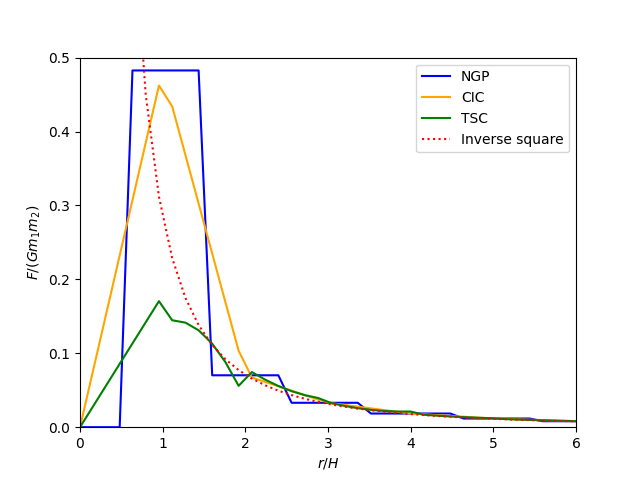
\includegraphics[width=\linewidth]{chapters/pm-method/img/pm-mass-assignment.png}
        \caption{Field strength calculated with the PM method using different assignment schemes (four-point finite difference).}
        \label{fig:pm-mass-assignment-field-strength}
    \end{subfigure}
    \caption{Approximation quality in the PM method.}
    \label{fig:pm-combined}
\end{figure}
The conclusion that can be drawn from \autoref{fig:pm-combined} is that, as expected, the TSC mass assignment scheme and the four-point finite difference yield the best results.

The field produced by the PM method using the ``poor man's'' potential solver is similar to the one obtained using the discretized Laplacian Green's function described above (see \autoref{fig:pm-poor-man-vs-laplacian}).
\begin{figure}[!ht]
    \centering
    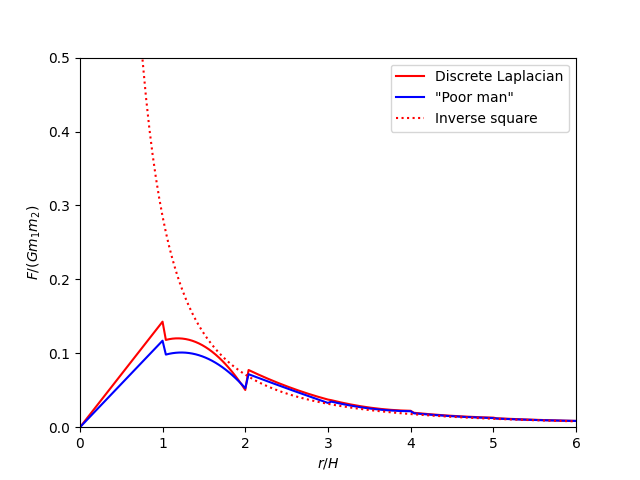
\includegraphics[scale=0.55]{chapters/pm-method/img/poor-man-vs-laplacian.png}
    \caption{Field obtained potential calculated by the ``Poor man's Poisson solver'' vs. when using \autoref{eq:dft-transformed-phi}.}
    \label{fig:pm-poor-man-vs-laplacian}
\end{figure}

\subsection{Global picture}\label{subsubsec:pm-global-picture}
To calculate the global approximation error of a PM simulation, we calculated the average of relative differences over all particles ($N=10{,}000$ in this case) between the forces produced by the PM method and the exact result obtained using the PP method.
More precisely, the error was defined as
\begin{equation}\label{eq:force-avg-relative-err}
    \frac{1}{N}\sum_{i} \frac{|\mathbf{F}_i^\text{approx.} - \mathbf{F}_i^\text{PP}|}{|\mathbf{F}_i^\text{PP}|}.
\end{equation}
The result for different grid resolutions is shown in \autoref{fig:pm-global-err-lap} ( $30 \leq N_g \leq 70$).
For this test, the particle positions were generated according to the uniformly decreasing density disk model.
\begin{figure}[!ht]
    \centering
    \begin{subfigure}[t]{0.48\textwidth}
        \centering
        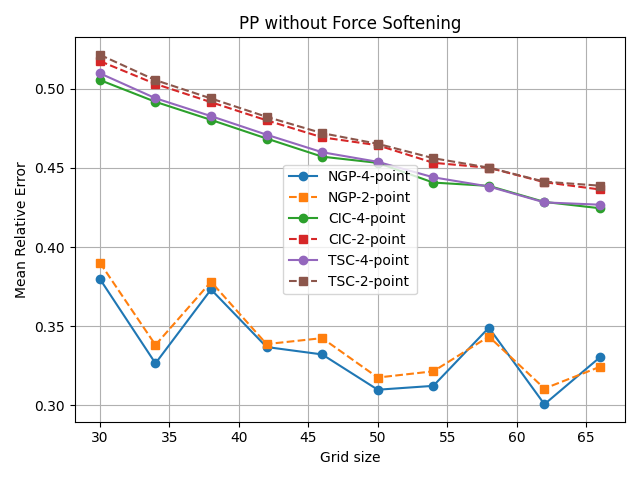
\includegraphics[width=\linewidth]{chapters/pm-method/img/pm-global-err.png}
        \caption{PP calculation without force softening.}
        \label{fig:pm-global-err-lap-no-soft}
    \end{subfigure}
    \hfill
    \begin{subfigure}[t]{0.48\textwidth}
        \centering
        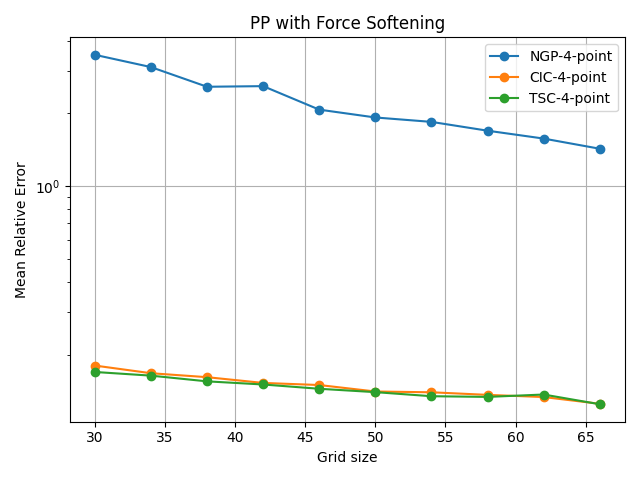
\includegraphics[width=\linewidth]{chapters/pm-method/img/pm-global-err-soft.png}
        \caption{PP calculation with force softening.}
        \label{fig:pm-global-err-lap-soft}
    \end{subfigure}
    \caption{Average force approximation error in the PM method (discrete Laplacian solver).}
    \label{fig:pm-global-err-lap}
\end{figure}
As can be seen in \autoref{fig:pm-global-err-lap-no-soft}, for each of the assignment schemes, the error is minimized for the four-point difference, as expected;
a more surprising result is that the errors are most significant for the TSC assignment scheme.
This paradox is easily explained by considering the graphs in \autoref{fig:pm-mass-assignment-field-strength}.
As can be seen there, the TSC assignment scheme gives rise to a force that accurately reproduces the inverse-square law force, but at the same time, it severely underestimates the force close to the source.
This behavior is expected since it stems from the mass of any individual particle being spread between multiple cells.
The CIC and NGP schemes, on the other hand, do not reproduce the actual force with the same level of accuracy, but the underestimation close to the source is not as severe as in the case of the TSC scheme.
In some applications, for instance, in the context of a galaxy simulation, this is a favorable feature of the TSC scheme.
The number of stars in a galaxy can be in the order of $10^{12}$ \cite{young2006andromeda}, whereas the number of particles in our tests is in the order of tens of thousands, giving an average of around $10^{12} / 10^{4} = 10^8$ of stars per particle.
Hence, it would be a grave mistake to model the force due to a single particle by the force due to a dimensionless point mass.
In such a case, it is a standard practice to use a softened gravitational force instead of the one given in \autoref{eq:law-of-uni-grav} \cite{10.1046/j.1365-8711.2000.03316.x}.
By using the TSC scheme, force softening is automatically included in the calculation.
It can be argued that obtaining the smoothness properties enjoyed by the higher-order assignment schemes should be treated as tangential to softening the force.
It is for this reason that Hockney and Eastwood introduce the notion of \textit{force sharpening} as an additional step in the PM method in \cite{Hockney1988}.
In this modified version of the PM method, the Poisson equation takes the form
\begin{equation*}
    \nabla^2 \phi_p = \rho_p^*,
\end{equation*}
where $\rho^*_p$ is obtained from the density $\rho_p$ by solving the following system
\begin{equation*}
    1+\frac{\rho^*_{p+1} - 2\rho^*_p + \rho^*_{p-1}}{8}
    = \rho_p,
\end{equation*}
where $p$ indexes the mesh points.
In this work, we do not investigate this matter further, nor do we implement this modification in our program.

Now we return to the test whose results are presented in \autoref{fig:pm-global-err-lap}.
In the light of the above discussion, it is more reasonable to compare the quality of the results of the PM method with a \textit{softened gravitational force} defined in \cite{Zhang_2019} as
\begin{equation}\label{eq:softened-force}
    \mathbf{F}^\textrm{soft}_{ij} = -G\frac{m_i m_j}{(r_{ij}^2 + \epsilon^2)^{3/2}}\mathbf{r}_{ij}.
\end{equation}
The relative difference between the softened forces and the PM-calculated ones is shown in \autoref{fig:pm-global-err-lap-soft}.
The \textit{softening length} in the PP method was set at $\epsilon = H$ in each run of the test so that it roughly matches the softening ``induced'' by the PM method (cf. \autoref{fig:pm-mass-assignment-field-strength}).
